\documentclass[10pt]{beamer}

\usetheme[progressbar=frametitle]{metropolis}
\usepackage{appendixnumberbeamer}

\usepackage{booktabs}
\usepackage[scale=2]{ccicons}
\usepackage[portuguese]{babel}

\usepackage{pgfplots}
\usepgfplotslibrary{dateplot}

\usepackage{xspace}
\newcommand{\themename}{\textbf{\textsc{metropolis}}\xspace}

\title{Geração Procedural de Terrenos para Jogos}
% \subtitle{A modern beamer theme}
\date{\today}
% \date{}
\author{João Carlos Becker}
% \institute{Center for modern beamer themes}
% \titlegraphic{\hfill\includegraphics[height=1.5cm]{logo.pdf}}

\begin{document}

\maketitle

% Qual o problema? porque é bom ter geração procedural terrenos
\section{Introdução}

\begin{frame}{Contextualização}
  \begin{itemize}
        \item Criar conteúdo para jogos manualmente exige muito esforço de trabalho
        \item Quanto maior o mundo virtual, tecnicamente mais tempo os jogadores irão explorar \cite{bevilacqua2009ferramenta}
    \end{itemize}
\end{frame}

\begin{frame}{Contextualização}
  \begin{figure}
		\centering
        \includegraphics[width=.8\textwidth]{img/intro/fc5terrain.png}
        \caption{Mapa de \alert{Far Cry 5}, \cite{Carrier2018farcry5}}
  \end{figure}
\end{frame}

\begin{frame}{Roteiro}
    \setbeamertemplate{section in toc}[sections numbered]
    \tableofcontents[hideallsubsections]
\end{frame}

\section{Requisitos}

% para algum ponto (x, z) precisa sempre gerar o mesmo y função (injetora) (consistência) (ser deterministico)
% (Variedade)
\begin{frame}{Requisitos}
    \begin{itemize}
        \item Determinismo, $ y = f(x, z) $
        \item \alert{Aleatoriedade}
    \end{itemize}
\end{frame}

\begin{frame}{Requisitos}
    \begin{figure}
		\centering
        \includegraphics[width=.8\textwidth]{img/intro/sssins.png}
        \caption{$ y = sin(x) + sin(z) $}
    \end{figure}  
\end{frame}



\begin{frame}{Aproximação do Mundo Real}
    \begin{itemize}
        \item Mostrar um método capaz de gerar um terreno para jogos
        \item Terrenos com relevos \alert{naturais}
    \end{itemize}
\end{frame}
% O que tem em um terreno (padrões fractais)

\begin{frame}{Aproximação do Mundo Real}
    \begin{figure}
		\centering
        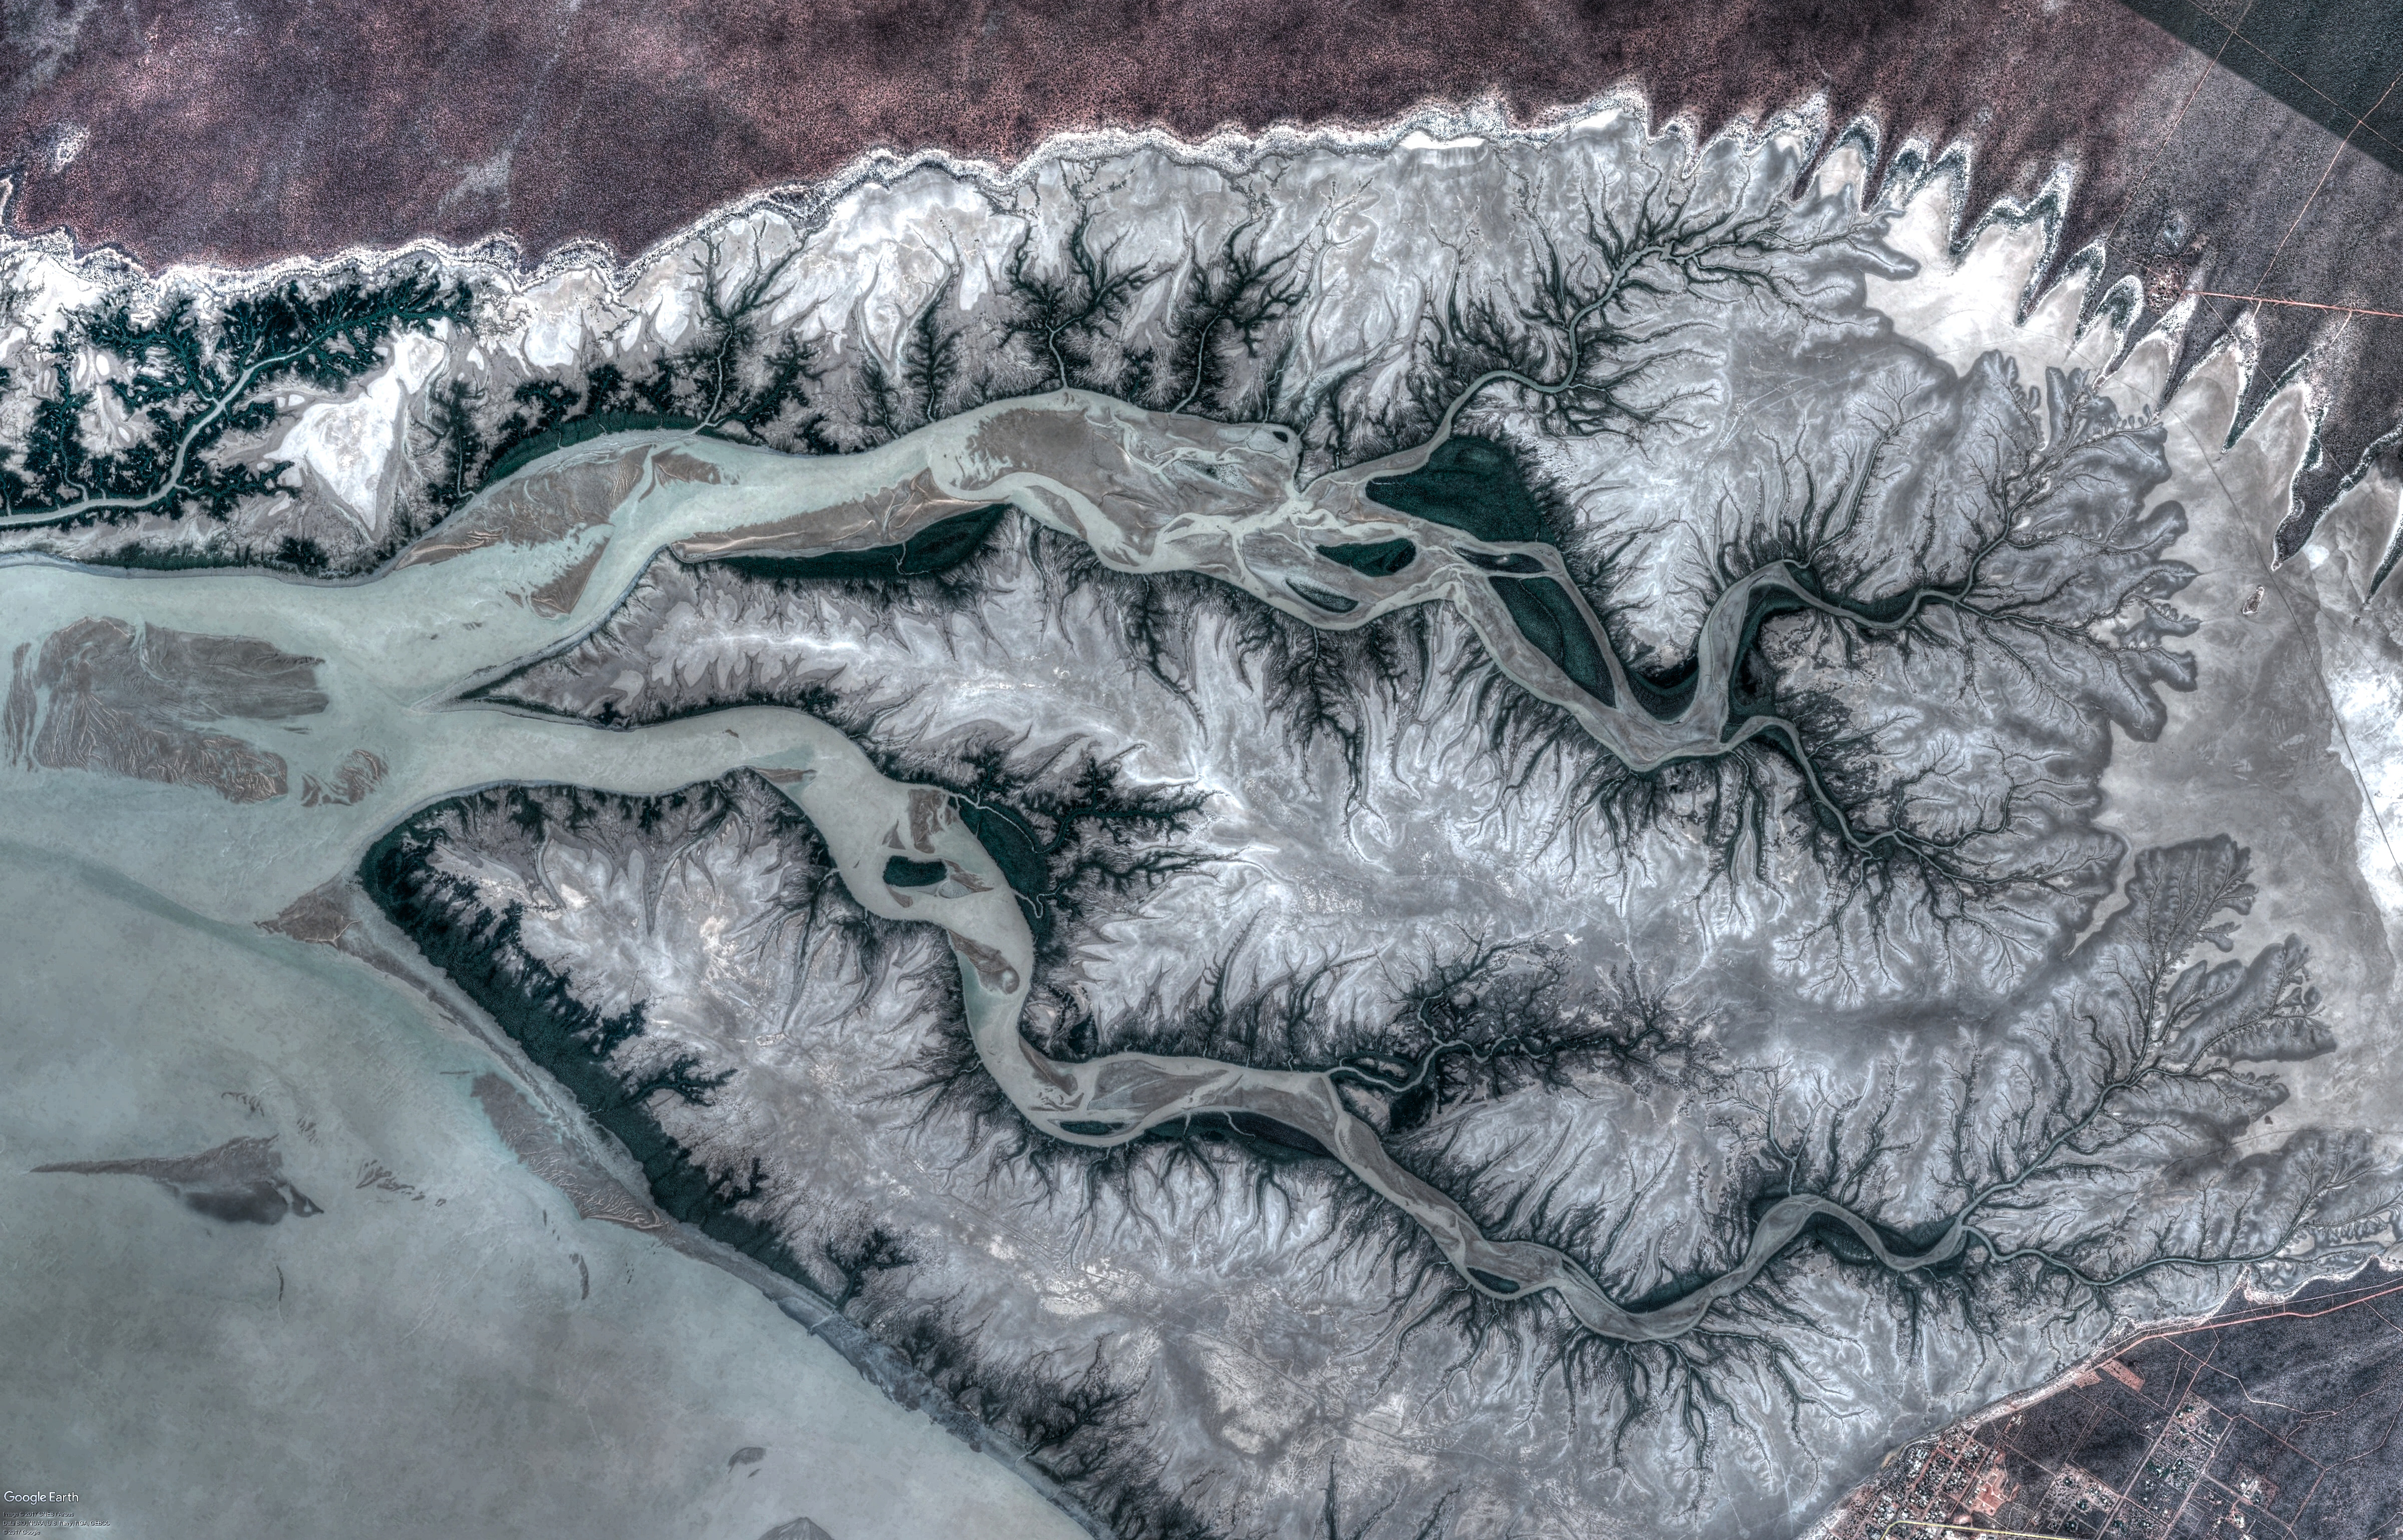
\includegraphics[width=.8\textwidth]{img/intro/derby.jpg}
        \caption{Erosão Fractal}
    \end{figure}
    imagem de \url{paulbourke.net/fractals/googleearth/}
\end{frame}

\section{Técnicas}
\metroset{block=fill}

\begin{frame}{Geração de Relevo}
    \begin{itemize}[<+- | alert@+>]
        \item \alert<6>{Ruído de Perlin}
        \item Divisões estocásticas
        \item Falhas geológicas
        \item Deposição de sedimentos
        \item Disposição do ponto médio
    \end{itemize}
\end{frame}

\begin{frame}{Noise}
    \begin{block}{Definição}
        \begin{itemize}
            \item Ponto: $Point \in \{ \mathbb{R}^3 \vee \mathbb{R}^2 \vee \mathbb{R}\} $
            \item $ -1 \leq noise(Point) \leq 1$
        \end{itemize}
    \end{block}
\end{frame}

\begin{frame}{Noise}
    \begin{figure}
		\centering
        \includegraphics[width=.7\textwidth]{img/explain/noiseRandom.png}
        \caption{\alert{Noise vs Random}, por \cite{shiffman2012nature}.}
    \end{figure}
\end{frame}

\begin{frame}{Noise}
    \begin{figure}
		\centering
        \includegraphics[width=.7\textwidth]{img/explain/1d2dnoise.png}
        \caption{\alert{1d and 2d Noise}, por \cite{shiffman2012nature}.}
    \end{figure}
    \begin{itemize}
        \item Complexidade para $n$ dimensões: $\mathcal{O}(2^n)$
    \end{itemize}
\end{frame}


\begin{frame}{Ruído de Perlin}
    \begin{itemize}
        \item Quantidade de oitavas: $\theta \in \mathbb{N}$
    \end{itemize}
    
    \begin{block}{Definição}
        $$perlinNoise(Point, \theta) = \sum_{t=0}^{t=\theta} \frac{Noise(Point \cdot 2^{t})}{2^{t}}$$
    \end{block}
\end{frame}


\begin{frame}{Ruído de Perlin}
    \begin{figure}
		\centering
        \includegraphics[width=.7\textwidth]{img/explain/perlin1d.png}
        \caption{Ruído de Perlin 1D, por \cite{elias2000perlin}.}
    \end{figure}
\end{frame}

\begin{frame}{Ruído de Perlin}
    \begin{figure}
		\centering
        \includegraphics[width=.7\textwidth]{img/explain/octaves1.png}
        \caption{$\theta = 1$.}
    \end{figure}
\end{frame}

\begin{frame}{Ruído de Perlin}
    \begin{figure}
		\centering
        \includegraphics[width=.7\textwidth]{img/explain/octaves4.png}
        \caption{$\theta = 4$.}
    \end{figure}
\end{frame}

\begin{frame}{Ruído de Perlin}
    \begin{figure}
		\centering
        \includegraphics[width=.7\textwidth]{img/explain/octaves16.png}
        \caption{$\theta = 16$.}
    \end{figure}
\end{frame}

\begin{frame}{Ruído de Perlin}
    \begin{block}{Caso de borda}
        $$\sum_{t=0}^{t=\theta} \frac{Noise(Point \cdot 2^{t})}{2^{t}}$$
        $$Noise(Point) = 1$$
        $$\sum_{t=0}^{t=\theta} \frac{1}{2^{t}} = 2^{-\theta} (2^{\theta +1}-1)$$
    \end{block}
\end{frame}


\begin{frame}{Ruído de Perlin}
    \begin{equation*}
        \begin{split}
            \visible<+->{max & = \lim_{\theta\to \infty} 2^{-\theta} (2^{\theta +1}-1) \\}
            \visible<+->{& = 2}
        \end{split}
    \end{equation*}
\end{frame}


\begin{frame}{Ruído de Perlin}
    \begin{figure}
		\centering
        \includegraphics[width=.7\textwidth]{img/explain/farLands.jpg}
        \caption{Limitações}
    \end{figure}
\end{frame}

% Mostrar o que é tesselation



\section{Contribuições da UFFS}

% Trabalho da Gabrielle
\begin{frame}{Geração Procedural de Cânions Baseado em Ruído de Perlin}
  \begin{itemize}
        \item A partir de uma classificação de características de cânions;
        \item As características mais comuns foram selecionadas.
    \end{itemize}
\end{frame}

\begin{frame}{Geração Procedural de Cânions Baseado em Ruído de Perlin}
  \begin{figure}
		\centering
        \includegraphics[width=.8\textwidth]{img/uffs/caract.png}
        \caption{Frequência de características nos cânions 
        \cite{gabrielle2016canion}.}
  \end{figure}
\end{frame}

\begin{frame}{Geração Procedural de Cânions Baseado em Ruído de Perlin}
  \begin{figure}
		\centering
        \includegraphics[width=.8\textwidth]{img/uffs/gabrielleDev.png}
        \caption{Soma das camadas para gerar Cânions}
  \end{figure}
\end{frame}

\begin{frame}{Geração Procedural de Cânions Baseado em Ruído de Perlin}
  \begin{figure}
		\centering
        \includegraphics[width=.65\textwidth]{img/uffs/gabrielleResultado.png}
        \caption{Resultado Final}
  \end{figure}
\end{frame}


% Meu trabalho
\begin{frame}{Geração de Terrenos com Biomas Distintos para Jogos}
    \begin{itemize}
        \item Implementação de relevo para 5 \alert{Biomas}
            \begin{itemize}
                \item Planícies
                \item Montanhas
                \item Vales
                \item Deserto
                \item Cânyons
            \end{itemize}
        \item Distribuição dos Biomas
        \item Suavização das fronteiras
    \end{itemize}
\end{frame}

\begin{frame}{Geração de Terrenos com Biomas Distintos para Jogos}
  \begin{figure}
		\centering
        \includegraphics[width=.8\textwidth]{img/uffs/bssMontains.png}
        \caption{Montanhas}
  \end{figure}
\end{frame}

\begin{frame}{Geração de Terrenos com Biomas Distintos para Jogos}
  \begin{figure}
		\centering
        \includegraphics[width=.8\textwidth]{img/uffs/biomesdistnoise.png}
        \caption{Distribuição de Biomas}
  \end{figure}
\end{frame}

\begin{frame}{Geração de Terrenos com Biomas Distintos para Jogos}
  \begin{figure}
		\centering
        \includegraphics[width=.8\textwidth]{img/uffs/256f4.png}
        \caption{Distribuição de Biomas}
  \end{figure}
\end{frame}

\begin{frame}{Geração de Terrenos com Biomas Distintos para Jogos}
  \begin{figure}
		\centering
        \includegraphics[width=.8\textwidth]{img/uffs/8b32.png}
        \caption{Frequência de Biomas = 8}
  \end{figure}
\end{frame}

\begin{frame}{Geração de Terrenos com Biomas Distintos para Jogos}
  \begin{figure}
		\centering
        \includegraphics[width=.8\textwidth]{img/uffs/16b32.png}
        \caption{Frequência de Biomas = 16}
  \end{figure}
\end{frame}

\begin{frame}{Geração de Terrenos com Biomas Distintos para Jogos}
  \begin{figure}
		\centering
        \includegraphics[width=.8\textwidth]{img/uffs/32b32.png}
        \caption{Frequência de Biomas = 32}
  \end{figure}
\end{frame}

\begin{frame}{Geração de Terrenos com Biomas Distintos para Jogos}
  \begin{figure}
		\centering
        \includegraphics[width=.8\textwidth]
        {img/uffs/interpolationArea/notinter.png}
        \caption{Fronteiras descontínuas}
  \end{figure}
\end{frame}

\begin{frame}{Geração de Terrenos com Biomas Distintos para Jogos}
  \begin{figure}
		\centering
        \includegraphics[width=.8\textwidth]
        {img/uffs/interpolationArea/showareanotinterpo.png}
        \caption{Casos de fronteiras}
  \end{figure}
\end{frame}

\begin{frame}{Geração de Terrenos com Biomas Distintos para Jogos}
  \begin{figure}
		\centering
        \includegraphics[width=.8\textwidth]
        {img/uffs/interpolationArea/showareainterpolating.png}
        \caption{Com interpolação}
  \end{figure}
\end{frame}

\begin{frame}{Geração de Terrenos com Biomas Distintos para Jogos}
  \begin{figure}
		\centering
        \includegraphics[width=.8\textwidth]{img/uffs/interpolationArea/interpolation.png}
        \caption{Com interpolação}
  \end{figure}
\end{frame}


% Trabalho do Fernando
\begin{frame}{Fernando}
  \begin{figure}
		\centering
        \includegraphics[width=.8\textwidth]
        {img/uffs/fernando/linearcosta.png}
        \caption{Costa linear.}
  \end{figure}
\end{frame}

\begin{frame}{Fernando}
  \begin{figure}
		\centering
        \includegraphics[width=.8\textwidth]{img/uffs/fernando/metodo.png}
        \caption{Método.}
  \end{figure}
\end{frame}

\begin{frame}{Fernando}
  \begin{figure}
		\centering
        \includegraphics[width=.8\textwidth]
        {img/uffs/fernando/costaorganica.png}
        \caption{Costa orgânica.}
  \end{figure}
\end{frame}

\section{Jogos com Conteúdo Procedural}

\begin{frame}{Spore}
    \begin{itemize}
        \item Gera planetas esféricos com relevo procedural
        \item Vegetação Procedural
    \end{itemize}
\end{frame}

\begin{frame}{Spore}
    \begin{figure}
  		\centering
        \includegraphics[width=.8\textwidth]{img/gameseg/spore.png}
        \caption{Spore, de \url{spore.fandom.com/wiki/Planet}}
    \end{figure}
\end{frame}

\begin{frame}{No man's sky}
    \begin{figure}
  		\centering
        \includegraphics[width=.8\textwidth]{img/gameseg/No-Mans-Sky.jpg}
        \caption{de \url{wccftech.com/no-mans-sky-xbox-one-release-june-29/}}
    \end{figure}
\end{frame}


% \begin{frame}{Far Cry 5}
%     \begin{itemize}
% 
%     \end{itemize}
% \end{frame}
% 


% Usado para parar a contagem na barra de progresso e paginação
\appendix

\begin{frame}[allowframebreaks]{Refêrencias}
    \bibliography{demo}
    \bibliographystyle{apalike}
\end{frame}

{\setbeamercolor{palette primary}{fg=black, bg=white}
    \begin{frame}[standout]
        Dúvidas?
    \end{frame}
}

\end{document}
